\section{Braking Module}

The Braking module implements the design specified in Sec.\ \ref{sec:Braking-Module-Design}. The hardware and software aspects of this module's implementation are discussed in this section. Figure \ref{fig:braking_pcb} shows a photo of the module after being populated and debugged.

\begin{figure}[H]
\centering
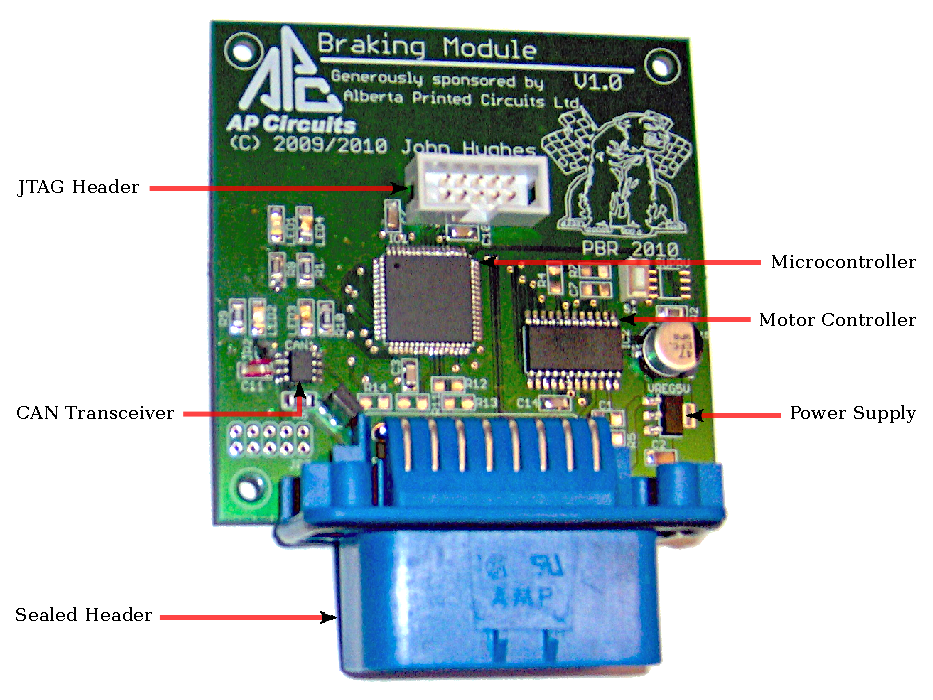
\includegraphics[scale=1]{implementation/figures/braking_pcb}
\caption{Photograph of the populated braking module PCB.}
\label{fig:braking_pcb}
\end{figure}

\subsection{Hardware}

The braking module implementation is the simplest of the four modules in terms of electrical design. Only one special hardware component is required, namely the stepper motor driver. This is summarized in Table \ref{table:braking_module_components}.

Figure \ref{fig:braking_pcb} shows a photograph of the completed braking module circuit board, with all components soldered on. The simplicity of the electrical design is reflected in the fact that no additional corrections (other than for the CAN transceiver) are required for the module to be 100\% operational.

\begin{table}
  \caption{List of components used by the braking module.}
  \centering
  \begin{tabular}{|c|c|c|}
    \hline 
    Part & Manufacturer & Part Number\tabularnewline 
    \hline \hline
    Stepper Motor Controller/Driver & Allegro Microsystems & A3967 \tabularnewline
    \hline
  \end{tabular}
  \label{table:braking_module_components}
\end{table}

\subsubsection{Stepper Motor Driver}

The Allegro Microsystems A3967 Micro-stepping Stepper Driver is used to drive the stepper motor. The A3967 integrates a micro-stepping controller with dual H-Bridge output stages into one package. The H-Bridge output transistors can supply up to $\pm\unit{750}{\milli\ampere}$ of current at up to \unit{30}{\volt} \cite{A3967}. The A3967 also provides a current-sensing feature for dynamically modifying the current supplied to the stepper motor. A current-sensing stepper motor driver allows us to adjust the current provided to the stepper motor by changing resistor values in the current-sense feedback loop. This allows us to remain flexible in terms of which stepper motor can be used in the final implementation.

\paragraph{Current Control}

\nomenclature{$R_{sense}$}{Value of the current sense resistors in the Braking Module's stepper motor circuit.}
\nomenclature{$I_{TRIP}max$}{Maximum current allowed to flow into the Braking Module's stepper motor before the PWM circuit shuts the output stage off.}

The current control feature of the A3967 works by sensing the current through a sense resistor, $R_{sense}$, and varies the duty cycle of a fixed off-time PWM circuit, which controls the output from the H-Bridge stages.

The value of the sense resistor is determined by an equation recommended in the manufacturer's data-sheet:

\begin{equation}
R_{sense}=\frac{0.5}{I_{TRIP}max}
\end{equation}
where $I_{TRIP}max$ is the maximum current allowed to flow into the motor before the PWM circuit shuts the output stage off.

The actual value of $R_{sense}$ used for bench testing the braking module is \unit{2}{\ohm}, which allows \unit{250}{\milli\ampere} output current. This is suitable for the stepper motor used in testing.

\subsection{Software}

The module software is entirely complete and all functionality is implemented. The brake module was the first to have it's software fully implemented, and served as the genesis for many of the low-level drivers.

\subsubsection{Bias Manager}

The bias library configures the CAN interface to listen for new adjustment and calibration requests over the network. Once a request arrives, the manager validates the request against the current state of the system and proceeds. 

\paragraph{Bias Adjustment Request}
\label{sec:impl_braking_bar}

The bias adjustment routine follows the flow chart illustrated in Fig. \ref{fig:design-braking-bias-adjustment}. Safety validation checks must be performed before the routine can get underway. 

First, the current front and rear brake pressures is requested from the pressure manager. If these pressures indicate the brakes are engaged, the procedure is aborted and an error message is broadcast over the CAN bus. Secondly, the current engine speed is captured over the CAN bus. If the engine RPM indicates the vehicle is in motion, the process is also aborted. Finally, the adjustment request is validated against the range of possible adjustments. If the request is out of range, the process is aborted and an error message is broadcast.

The number of offset steps $steps_{offset}$ is calculated from the desired bias position ``$pos_{desired}$'' and the current bias position. The manager is aware of how many steps are required to adjust the bias by one-half a percentage (``$steps_{half}$''). Moving the balance bar to the right increases the front-to-rear bias ratio. Therefore:

\[
steps_{offset} = (pos_{desired} - pos_{current}) * 2 * steps_{half}
\]

If this value is negative, the stepper motor is turned clockwise to move the balance bar left. Otherwise, it is turned counter-clockwise to move the balance bar right. Once completed, the bias manager broadcasts a success message over the bus. If an error occurs during operation, such as an end-of-travel switch being triggered, an error message is broadcast detailing the problem. 

\paragraph{Bias Calibration}

The bias calibration routine follows the flow chart illustrated in Fig. \ref{fig:brake_bias_calibration_flow}. Like the bias adjustment request, the bias manager ensures the brakes are not engaged before proceeding.

The calibration routine requests that it be interrupted when either end-of-travel switch is triggered. It then uses the stepper interface to rotate the balance bar to the left, until an interrupt occurs. The stepper interface is then used to rotate the balance bar all the way to the right, one step at a time. An index is incremented with each step. Once the right end-of-travel is reached, the bias manager stores the new number of steps required to travel the full-scale of the balance bar. It then divides the steps travelled by two and rotates the bar back by this many steps, thus centering the bar. Finally, the adjustment procedure is invoked to restore the original bias ratio, assuming the current bias is 50/50.

\subsubsection{Pressure Manager}

The pressure manager has two main tasks: to output the current brake pressure over the bus at a periodic interval, and to respond to requests for calibration. It uses the CAN interface to listen for calibration requests, much like the bias manager. 

\paragraph{Periodic Pressure Output}

The pressure manager uses an on-board timer on the micro-controller to periodically (every \unit{100}{\milli\second}) interrupt code execution to sample the current pressure with the ADC interface, and to broadcast it over the bus. 

Each pressure value is a 10-bit number stored in an unsigned 16-bit number, so two CAN packets are broadcast:one for the front, and one for the rear. The first two data bytes correspond to the \emph{most significant byte} (MSB) and \emph{least significant byte} (LSB) of the current pressure reading. This is followed by the MSB and LSB of the minimum calibrated pressure, and the MSB and LSB of the maximum calibrated pressure.

\paragraph{Pressure Calibration}

The pressure calibration routine follows the flow chart illustrated in Fig. \ref{fig:brake_pressure_calibration_flow}. The vehicle must not be in motion while this takes place, so a check for vehicle speed similar to that in Sec. \ref{sec:impl_braking_bar} is carried out. 

The pressure manager will broadcast a packet indicating that it is requires the driver to remove their foot from the brake. The driver then indicates this is done by pushing the diagnostic button on the driver interface. This causes a reply packet to be broadcast back to the pressure manager. Once received, the pressure manager uses the ADC interface to sample the front and rear pressures and stores them in a temporary value.

A similar routine occurs for the maximum pressure value. Once received, the calibration function validates the temporary values it has sampled. The rules that must be followed are:

\begin{itemize}
\item The minimum pressure must be less than the maximum pressure; and
\item There must be a minimum pressure difference of 500 psi between the minimum and maximum pressures.
\end{itemize}

If the samples pass this validation, they are stored as new calibration values. Otherwise, an error message is broadcast.

\subsubsection{Stepper Driver}

The stepper driver drives the discrete control lines required by the A3967 to enable stepper operation. The interface to the module software is simple: a single function allows the software to request the stepper move a particular number of steps in a particular direction.

The function toggles the direction line of the A3967 based on the desired direction. It then triggers the step signal to advance the motor. This process repeats for each step desired. 

The A3967 has strict timing requirements for how long the signal lines must be held and what sort of delay is required between signal changes. We cannot rotate the bar too fast because of the inertia of the balance bar. The driver introduces an automatic 50 ms delay between steps, allowing for a maximum rotation speed of 50 RPM for a 24-tooth stepper motor.
